\chapter{SYCO: SYstematic testing tool for Concurrent Objects}

SYCO es una de las herramientas implementadas sobre el lenguaje ABS que permite el testing de programas concurrentes escritos en este lenguaje. La idea de SYCO es que, a partir del código de un programa, el programador pueda saber de antemano las posibles ejecuciones del programa además de conocer si el programa presenta posibles situaciones de deadlock.\\

El núcleo de SYCO incluye implementaciones de técnicas de partial-order reduction que permiten la evaluación de ramas redundantes como las que se nos han presentado al principio de este trabajo en algunos ejemplos.\\

A través de una interfaz web, uno puede obtener visualmente el resultado que SYCO genera sobre el código proporcionado.\\

Veamos algunos ejemplos de uso sobre el código ABS generado a partir de un código en CABS.\\

\begin{lstlisting}
int var;

int main() {
    thread f(1);
    thread f(2);
    return 0;
}

void f(int value) {
    var = value;
}
\end{lstlisting}

En este ejemplo tenemos que la función $main$ lanza dos hilos que ejecutarán la función $f$ dando como posibles resultados finales $var = 1$ y $var = 2$. La traducción a ABS quedaría, resumiendo parte de la traducción que no es necesaria para este ejemplo, como:

\begin{lstlisting}
module Cabs;
import * from ABS.StdLib;

interface GLOBAL {
  Int getvar();
  Unit setvar(Int val);
  Unit initialize();
}

class GlobalVariables() implements GLOBAL {
  Int var = 0;
  Unit initialize() {
  }
  Int getvar() {
  	return var;
  }
  Unit setvar(Int val) {
  	var = val;
  }
}

interface Intf {
  Unit f(Int value);
}
interface Intmain {
  Int main();
}

class Impf(GLOBAL globalval) implements Intf {
  Unit f(Int value) {
  	await globalval!setvar(value);
  }
}

class Impmain(GLOBAL globalval) implements Intmain {
  Int main() {
    Intf aux_var_0 = new Impf(globalval);
    Int aux_var_1 = 1;
    aux_var_0!f(aux_var_1);
    Intf aux_var_2 = new Impf(globalval);
    Int aux_var_3 = 2;
    aux_var_2!f(aux_var_3);
    Int aux_var_4 = 0;
    return aux_var_4;
  }
}

{
  GLOBAL globalval = new GlobalVariables();
  await globalval!initialize();
  Intmain prog = new Impmain(globalval);
  await prog!main();
}

\end{lstlisting}
Y el resultado que nos proporciona la herramienta SYCO es:
\begin{verbatim}
Independence constraints generated in 908 ms.
Number of executions: 2
Total time: 5
Total number of states explored during 2 executions: 16
Total number of tasks executed during 2 executions: 7
Execution 1, number of tasks: 6
(Click here to see the sequence diagram)
- State:
|------object(1,'GlobalVariables',[field(var,2)])
|------object(2,'Impmain',[field(globalval,ref(1))])
|------object(3,'Impf',[field(globalval,ref(1))])
|------object(4,'Impf',[field(globalval,ref(1))])
|------object(main,main,[])
- Trace: |------'Time: 0, Object: main, Task: 0:main'
|------'Time: 1, Object: GlobalVariables_1, Task: 1:initialize'
|------'Time: 2, Object: 0:main(54), Task: 0:main(54)'
|------'Time: 3, Object: Impmain_2, Task: 3:main'
|------'Time: 4, Object: 0:main(56), Task: 0:main(56)'
|------'Time: 5, Object: Impf_3, Task: 5:f'
|------'Time: 6, Object: GlobalVariables_1, Task: 7:setvar'
|------'Time: 7, Object: Impf_3, Task: 5:f(34)'
|------'Time: 8, Object: Impf_4, Task: 6:f'
|------'Time: 9, Object: GlobalVariables_1, Task: 9:setvar'
|------'Time: 10, Object: Impf_4, Task: 6:f(34)'
Execution 2, number of tasks: 6
(Click here to see the sequence diagram)
- State:
|------object(1,'GlobalVariables',[field(var,1)])
|------object(2,'Impmain',[field(globalval,ref(1))])
|------object(3,'Impf',[field(globalval,ref(1))])
|------object(4,'Impf',[field(globalval,ref(1))])
|------object(main,main,[])
- Trace: |------'Time: 0, Object: main, Task: 0:main'
|------'Time: 1, Object: GlobalVariables_1, Task: 1:initialize'
|------'Time: 2, Object: 0:main(54), Task: 0:main(54)'
|------'Time: 3, Object: Impmain_2, Task: 3:main'
|------'Time: 4, Object: 0:main(56), Task: 0:main(56)'
|------'Time: 5, Object: Impf_3, Task: 5:f'
|------'Time: 6, Object: Impf_4, Task: 6:f'
|------'Time: 7, Object: GlobalVariables_1, Task: 9:setvar'
|------'Time: 8, Object: GlobalVariables_1, Task: 7:setvar'
|------'Time: 9, Object: Impf_3, Task: 5:f(34)'
|------'Time: 10, Object: Impf_4, Task: 6:f(34)'
\end{verbatim}
donde podemos ver las dos trazas obtenidas.\\

Para un ejemplo más elaborado como es
\begin{lstlisting}
int var;
int var2;

int main() {
    thread f();
    thread g();
    return 0;
}

void f() {
    var = 1;
    var = 2;
}

void g() {
    var2 = 10 * var + var;
}
\end{lstlisting}

cuya traducción ``resumida'' es

\begin{lstlisting}
module Cabs;
import * from ABS.StdLib;

interface GLOBAL {
  Int getvar();
  Unit setvar(Int val);
  Int getvar2();
  Unit setvar2(Int val);
  Unit initialize();
}
class GlobalVariables() implements GLOBAL {
  Int var = 0;
  Int var2 = 0;
  Unit initialize() {
  }
  Int getvar() {
    return var;
  }
  Unit setvar(Int val) {
    var = val;
  }
  Int getvar2() {
    return var2;
  }
  Unit setvar2(Int val) {
    var2 = val;
  }
}

interface Intf {
  Unit f();
}

interface Intg {
  Unit g();
}

interface Intmain {
  Int main();
}

class Impf(GLOBAL globalval) implements Intf {
  Unit f() {
    Int aux_var_0 = 1;
    await globalval!setvar(aux_var_0);
    Int aux_var_1 = 2;
    await globalval!setvar(aux_var_1);
  }
}

class Impg(GLOBAL globalval) implements Intg {
  Unit g() {
    Int aux_var_2 = 10;
    Int aux_var_3 = await globalval!getvar();
    Int aux_var_4 = (aux_var_2 * aux_var_3);
    Int aux_var_5 = await globalval!getvar();
    Int aux_var_6 = (aux_var_4 + aux_var_5);
    await globalval!setvar2(aux_var_6);
  }
}

class Impmain(GLOBAL globalval) implements Intmain {
  Int main() {
    Intf aux_var_7 = new Impf(globalval);
    aux_var_7!f();
    Intg aux_var_8 = new Impg(globalval);
    aux_var_8!g();
    Int aux_var_9 = 0;
    return aux_var_9;
  }
}

{
  GLOBAL globalval = new GlobalVariables();
  await globalval!initialize();
  Intmain prog = new Impmain(globalval);
  await prog!main();
}
\end{lstlisting}

podemos rápidamente concluir cuáles son los 6 posibles resultados finales de la ejecución del código.\\


\begin{figure}[h]
  \centering
  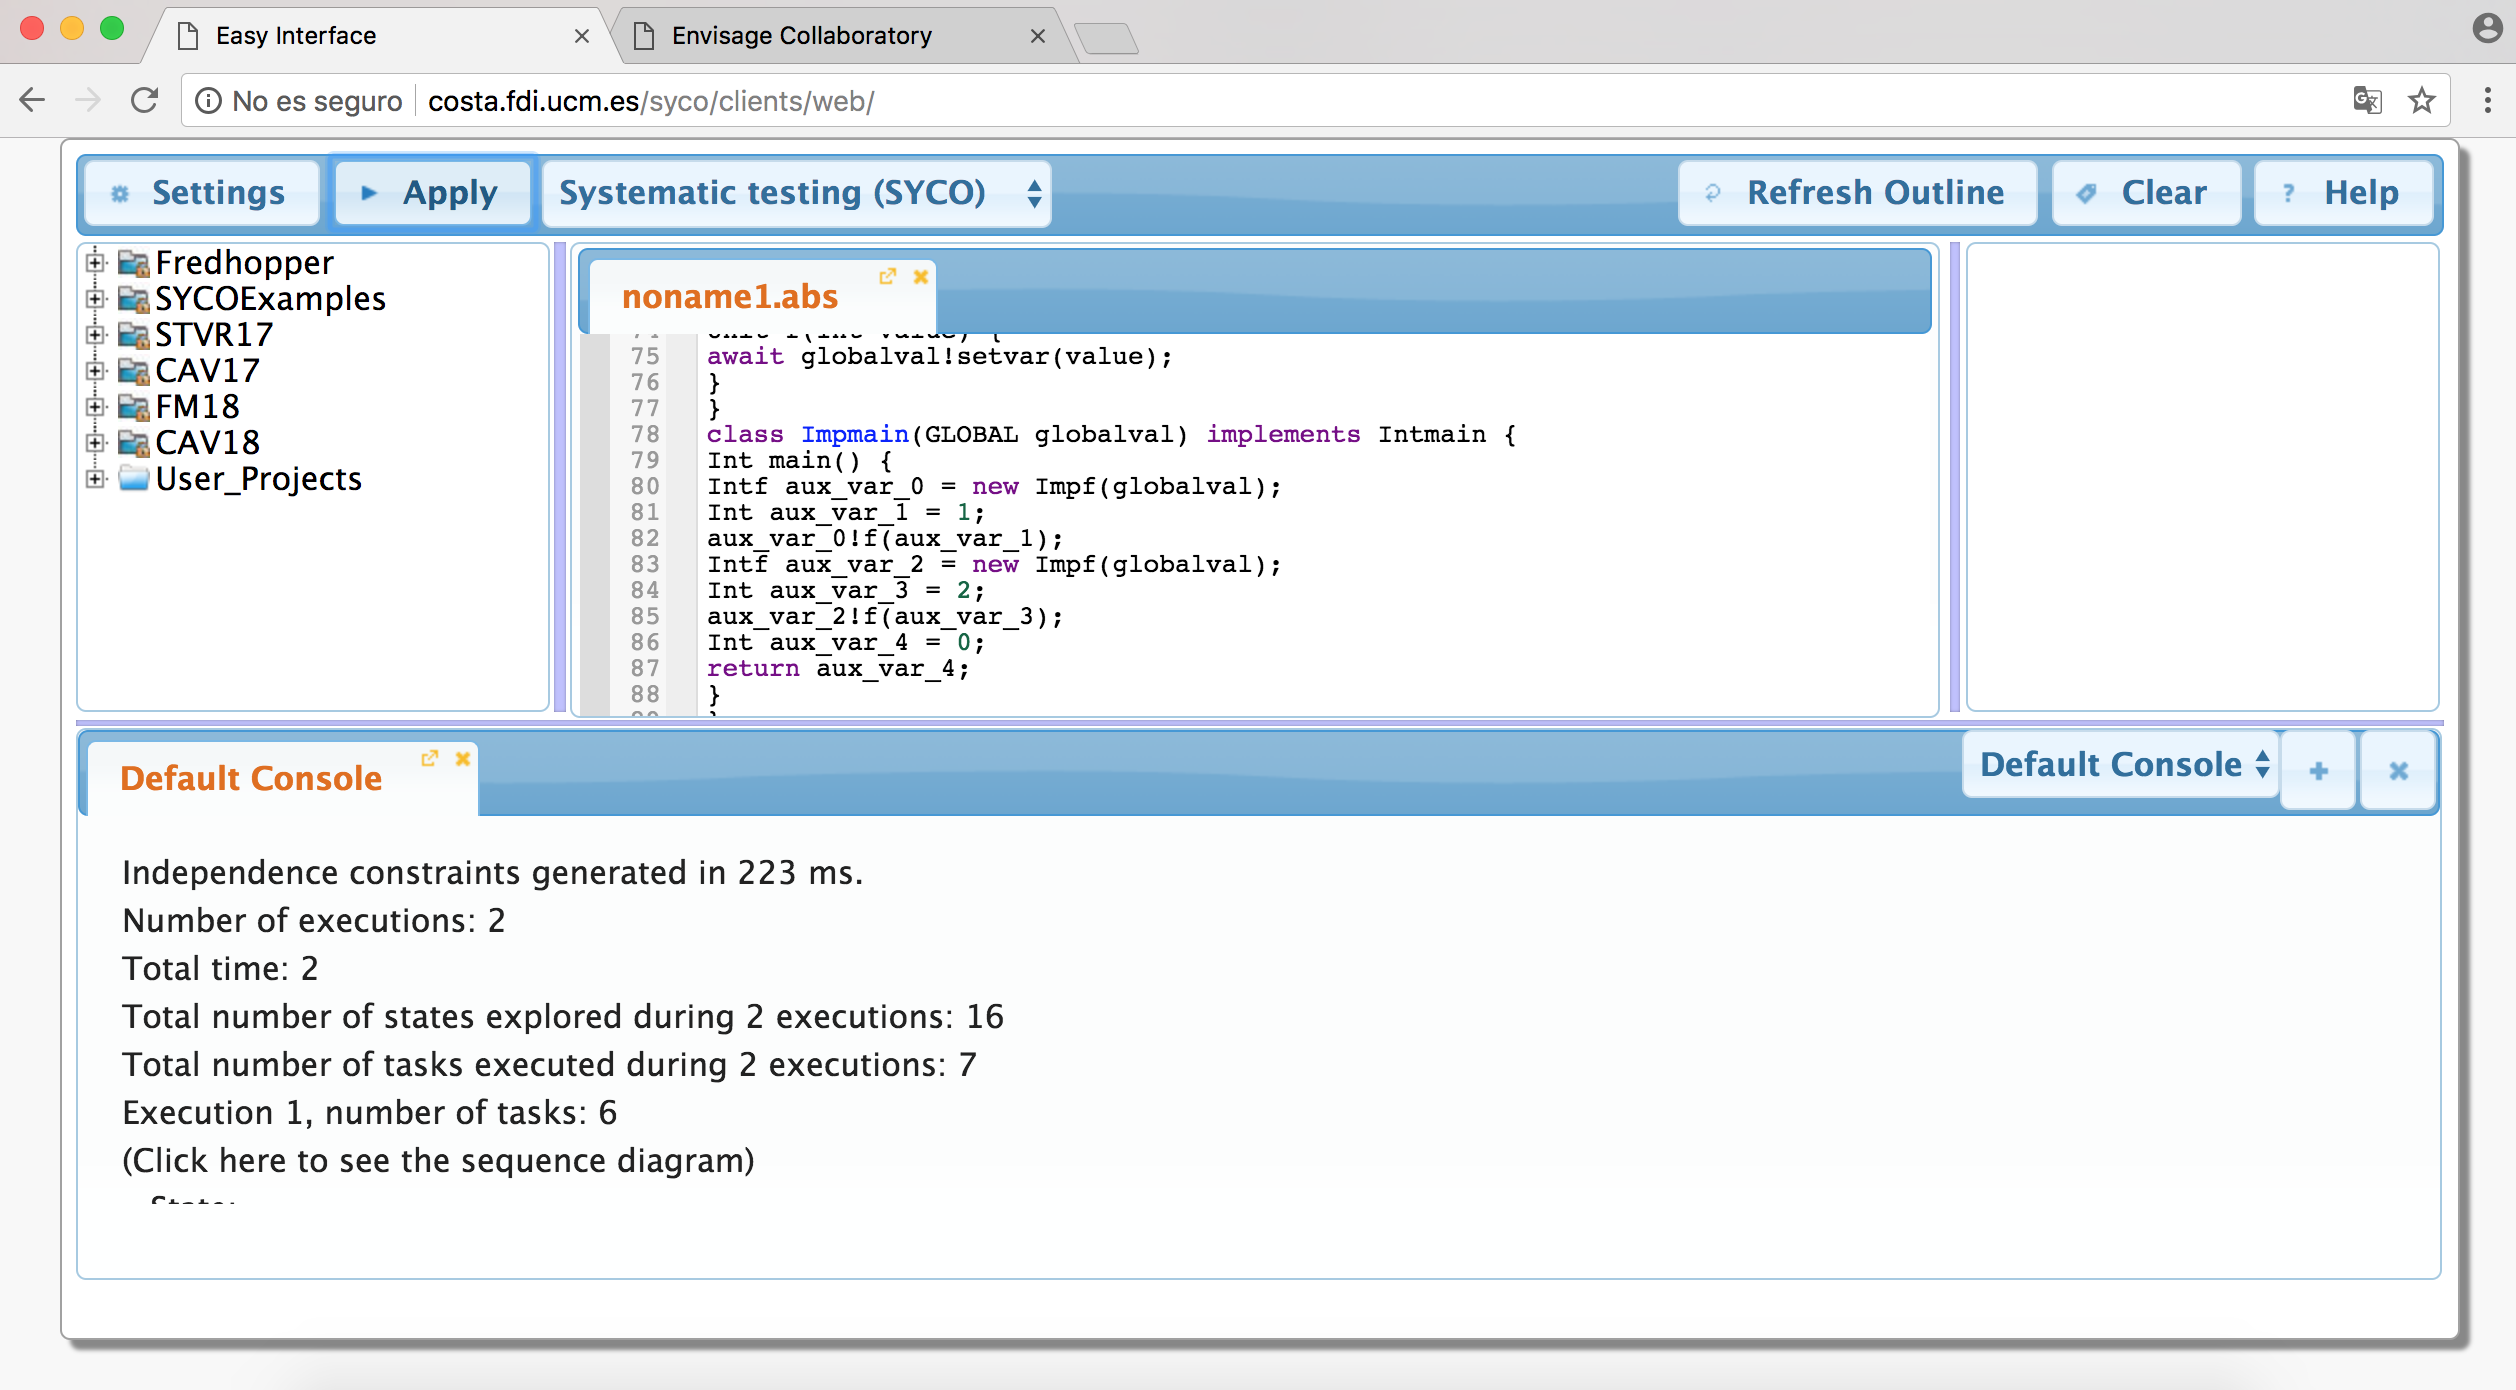
\includegraphics[scale=0.36]{syco.png}
  \caption{Captura de la herramienta SYCO.}
\end{figure}
